\title{Crafting Unit Tests}
%\author{
%  Olivier Albiez \texttt{@OlivierAlbiez} \\
%  Yann Danot \texttt{@ydannot}
%}


\newcommand{\punchline}[2]{%
  \begin{quote}{\includegraphics[width=0.8cm]{common/quote}}
    #2
    \begin{flushright}
      \tiny{---#1}
    \end{flushright}
  \end{quote}
}


\newcommand\cadre{
  \begin{scope}
    \fill[white,draw=gray!20!white, very thin] (-2, -0.5) rectangle (8, 6.5);
  \end{scope}
}

\newcommand\etoepart{
  \begin{scope}
    \clip (0, 4) rectangle (6, 6);
    \fill[gray!20!white] (0,0) -- (6,0) -- (3,6) -- cycle;
    \node (etoe) at (3,4.5) {E2E};
  \end{scope}
}

\newcommand\integpart{
  \begin{scope}
    \clip (0, 2) rectangle (6,3.8);
    \fill[gray!20!white] (0,0) -- (6,0) -- (3,6) -- cycle;
    \node (integ) at (3,2.5) {Integration};
  \end{scope}
}

\newcommand\unitpart{
  \begin{scope}
    \clip (0, 0) rectangle (6,1.8);
    \fill[gray!20!white] (0,0) -- (6,0) -- (3,6) -- cycle;
    \node (unit) at (3,0.5) {Unit};
  \end{scope}
}

\newcommand\drawsystem{
\begin{scope}
  [
    link/.style = {
      Latex[round]-Latex[round],
      thick,
      shorten <=1mm,
      shorten >=1mm
    },
    application/.style = {
      rectangle,
      rounded corners=1mm,
      draw=blue!50,
      fill=blue!20,
      thin,
      minimum width=2cm,
      minimum height=1cm,
    },
    db/.style = {
      cylinder,
      shape border rotate=90,
      draw=blue!50,
      fill=blue!20,
      thin,
      minimum width=1.5cm,
    },
    bus/.style = {
      cylinder,
      draw=blue!50,
      fill=blue!20,
      thin,
      minimum height=1.5cm,
    },
    internet/.style = {
      cloud,
      draw=black!50,
      fill=gray!20,
      thin,
      minimum width=1.5cm,
      minimum height=0.75cm,
    },
  ]

  \node[application] (frontend)                          {Frontend};
  \node[application] (backend)  [below=of frontend]      {Backend};
  \node[db]          (db)       [below left=of backend]  {DB};
  \node[db]          (fs)       [below right=of backend] {Files};
  \node[bus]         (bus)      [left=of backend]        {Bus};
  \node[internet]    (internet) [right=of backend]       {};
  \node[application] (partners) [right=of internet]      {Partners};

  \draw [link] (frontend) -- (backend);
  \draw [link] (backend) -- (db);
  \draw [link] (backend) -- (fs);
  \draw [link] (backend) -- (bus);
  \draw [link] (backend) -- (internet);
  \draw [link] (internet) -- (partners);
\end{scope}
}


\begin{document}


\frame{\titlepage}

%Les objectifs de la formation :
%– Etre sensibilisé à l’écriture des tests
%– Apprendre à écrire des vrais tests unitaires (TU)
%– Ecrire des tests lisibles et maintenables

\section{Definitions}
\begin{frame}{What do you mean by test ?}
  \begin{center}
    \includegraphics<2>[width=0.8\textwidth]{images/test-alpha}
  \end{center}

  \note{
    Word cloud basé sur l’article wikipedia \url{https://en.wikipedia.org/wiki/Software_testing}
  }
\end{frame}


\begin{frame}{What about unit tests ?}
  \begin{center}
    \includegraphics<2>[width=0.8\textwidth]{images/tu-alpha}
  \end{center}

  \note{Faire le tour des avis sur la question.}
\end{frame}


\begin{frame}{What about unit tests ?}
  \singlequote{Wikipedia}{
    In computer programming, unit testing is a software testing method by which individual \alert{units} of source \alert{code}, sets of one or more computer program \alert{modules} together with \alert{associated control data}, \alert{usage procedures}, and \alert{operating procedures}, are tested to determine whether they are fit for use.
  }
\end{frame}


\begin{frame}{What about unit tests ?}
  \begin{center}
    \begin{tikzpicture}
      \drawsystem
    \end{tikzpicture}
  \end{center}
\end{frame}


\begin{frame}{What about unit tests ?}
  \begin{center}
    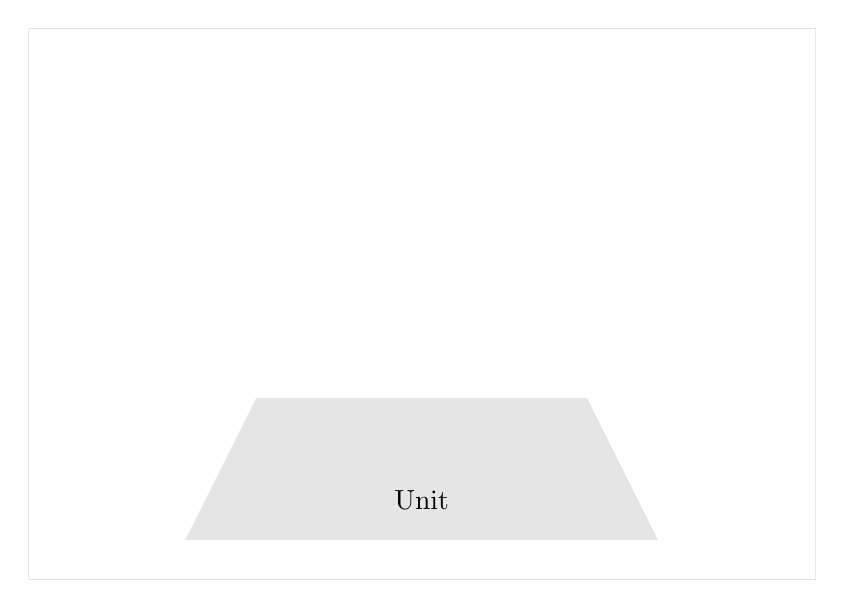
\begin{tikzpicture}
      \cadre
      \unitpart
    \end{tikzpicture}
  \end{center}
\end{frame}


\begin{frame}{What about unit tests ?}
  \begin{center}
    \begin{tikzpicture}
      \drawsystem
    \end{tikzpicture}
  \end{center}
\end{frame}


\begin{frame}{What about unit tests ?}
  \begin{center}
    \begin{tikzpicture}
      \drawsystem
      \begin{scope}
        \foreach \x in {1,...,10} {
          \fill[alert_color] ($ (frontend) + (0.8*rand,0.4*rand) $) circle [radius=0.6mm,];
          \fill[alert_color] ($ (backend) + (0.8*rand,0.4*rand) $) circle [radius=0.6mm,];
        }
      \end{scope}
    \end{tikzpicture}
  \end{center}

  \note{Si on prend une application classique, qu’appelle-t-on UT. Un test passant par plusieurs classes mais restant isolé du monde extérieur à l’appli est-il considéré comme un UT?}
\end{frame}


\begin{frame}{What about unit tests ?}
  \begin{center}
    \begin{tikzpicture}
      \drawsystem
      \begin{scope}[decoration=snake,alert_color,ultra thick]
        \foreach \x in {-0.7,0,0.7} {
          \draw [decorate] ($ (frontend) + (\x,0.4) $) -- ($ (frontend) + (\x,-0.4) $);
          \draw [decorate] ($ (backend) + (\x,0.4) $) -- ($ (backend) + (\x,-0.4) $);
        }
      \end{scope}
    \end{tikzpicture}
  \end{center}
\end{frame}


\begin{frame}{What about unit tests ?}
  \begin{center}
  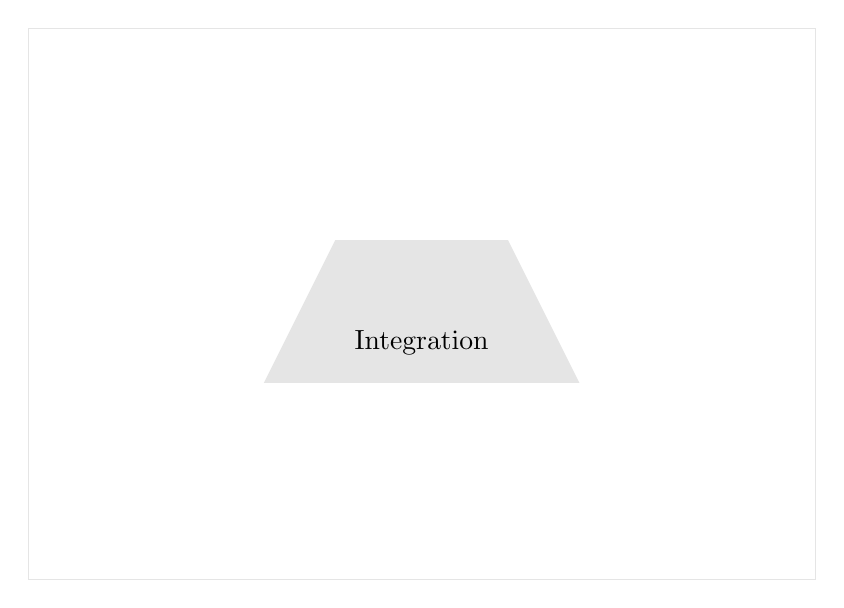
\begin{tikzpicture}
    \cadre
    \integpart
  \end{tikzpicture}
  \end{center}
\end{frame}


\begin{frame}{What about unit tests ?}
  \begin{center}
    \begin{tikzpicture}
      \drawsystem
    \end{tikzpicture}
  \end{center}
\end{frame}


\begin{frame}{What about unit tests ?}
  \begin{center}
    \begin{tikzpicture}
      \drawsystem
      \begin{scope}[decoration={snake,amplitude=1},draw=alert_color,ultra thick]
        \draw [decorate] (backend.north) -- (db.center) ;
      \end{scope}
    \end{tikzpicture}
  \end{center}
\end{frame}


\begin{frame}{What about unit tests ?}
  \begin{center}
    \begin{tikzpicture}
      \drawsystem
      \begin{scope}[decoration={snake,amplitude=1},draw=alert_color,ultra thick]
        \draw [decorate] (frontend.70) -- (backend.100) -- (bus.center) ;
      \end{scope}
    \end{tikzpicture}
  \end{center}
\end{frame}


\begin{frame}{What about unit tests ?}
  \begin{center}
  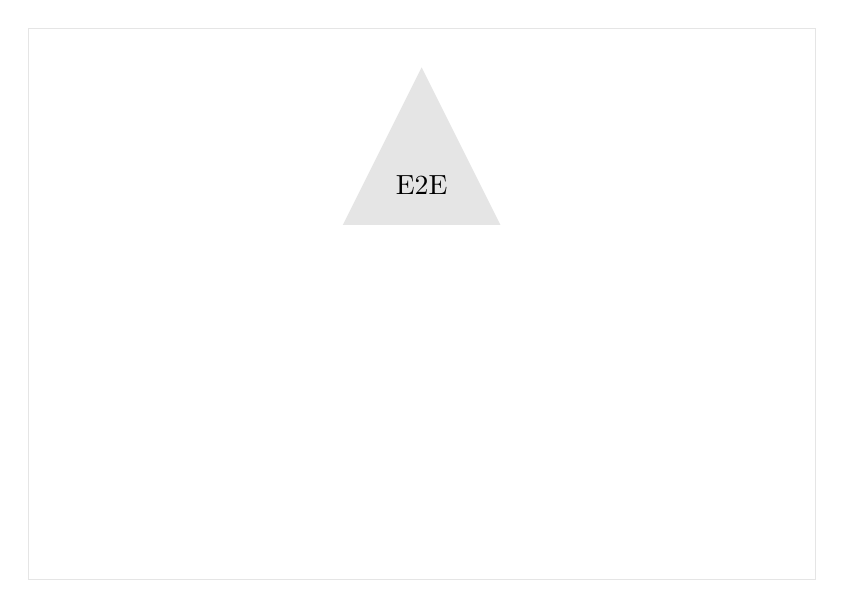
\begin{tikzpicture}
    \cadre
    \etoepart
  \end{tikzpicture}
  \end{center}
\end{frame}


\begin{frame}{What about unit tests ?}
  \begin{center}
    \begin{tikzpicture}
      \drawsystem
    \end{tikzpicture}
  \end{center}
\end{frame}


\begin{frame}{What about unit tests ?}
  \begin{center}
    \begin{tikzpicture}
      \drawsystem
      \begin{scope}[decoration={snake,amplitude=1},draw=alert_color,ultra thick]
        \draw [decorate] (frontend.130) -- (backend.222) -- (db.center) ;
      \end{scope}
    \end{tikzpicture}
  \end{center}
\end{frame}


\begin{frame}{What about unit tests ?}
  \begin{center}
    \begin{tikzpicture}
      \drawsystem
      \begin{scope}[decoration={snake,amplitude=1},draw=alert_color,ultra thick]
        \draw [decorate] (frontend.130) -- (backend.222) -- (db.center) ;
        \draw [decorate] (frontend.north) -- (backend.center) -- (fs.center) ;
      \end{scope}
    \end{tikzpicture}
  \end{center}
\end{frame}


\begin{frame}{What about unit tests ?}
  \begin{center}
    \begin{tikzpicture}
      \drawsystem
      \begin{scope}[decoration={snake,amplitude=1},draw=alert_color,ultra thick]
        \draw [decorate] (frontend.130) -- (backend.222) -- (db.center) ;
        \draw [decorate] (frontend.north) -- (backend.center) -- (fs.center) ;
        \draw [decorate] (bus.center) -- (backend.west) -- (db.center) ;
        \draw [decorate] (frontend.70) -- (backend.east) -- (partners.center) ;
      \end{scope}
    \end{tikzpicture}
  \end{center}
\end{frame}

\section{Test strategy}
\section{Test strategy}


\begin{frame}{Test pyramid}
  \begin{center}
  \begin{tikzpicture}
    \cadre
    \etoepart
    \integpart
    \unitpart
    \node [alert_color] at($ (etoe.center) + (-1.4, 0)$)  {10};
    \node [alert_color] at($ (integ.center) + (-2.5, 0)$) {100};
    \node [alert_color] at($ (unit.center) + (-3.6, 0)$)  {10000};
  \end{tikzpicture}
  \end{center}
\end{frame}


\begin{frame}{Functional vs Technical tests}
  \begin{center}
  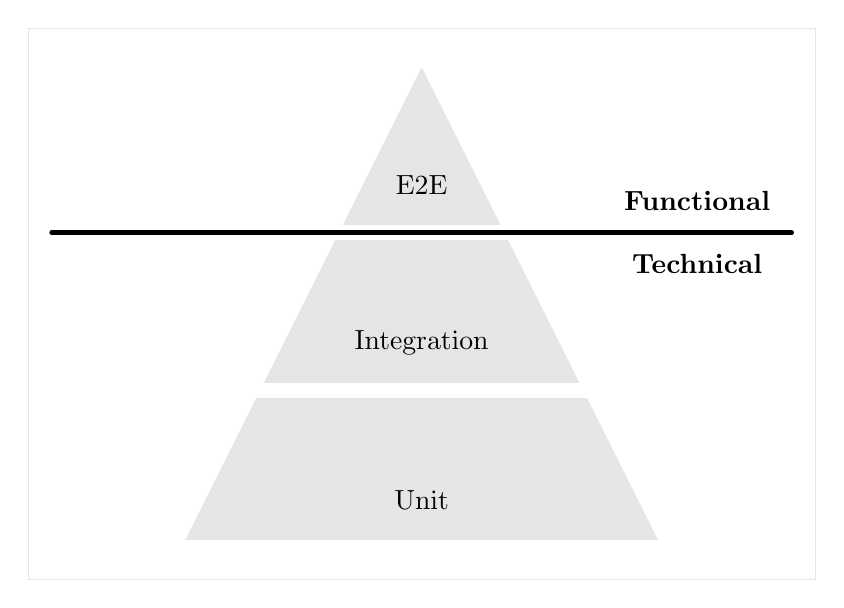
\begin{tikzpicture}
    \cadre
    \etoepart
    \integpart
    \unitpart
    \draw[ultra thick,line cap=round] (-1.7,3.9) -- (7.7,3.9);
    \node at(6.5,4.3) {\alert{\textbf{Functional}}};
    \node at(6.5,3.5) {\alert{\textbf{Technical}}};
  \end{tikzpicture}
  \end{center}
\end{frame}


\begin{frame}{Functional vs Technical tests}
  \begin{center}
  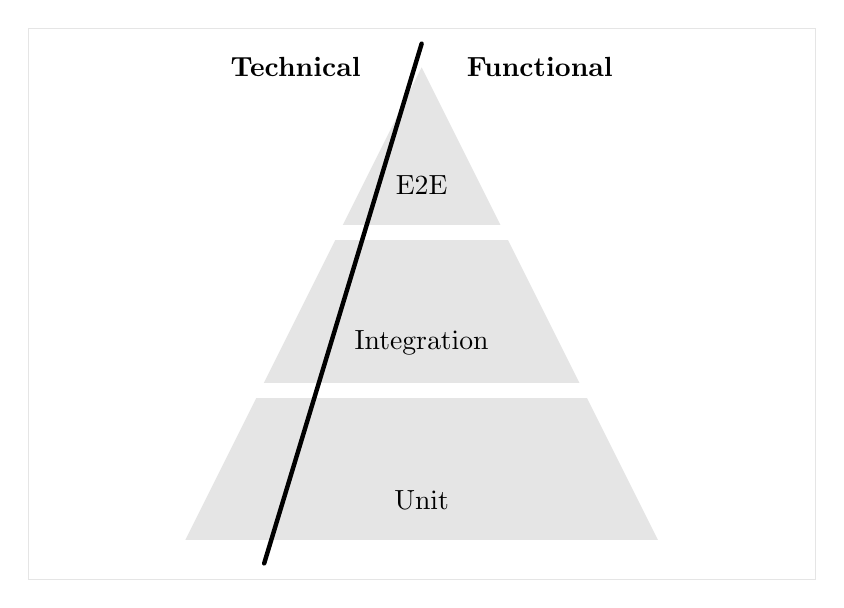
\begin{tikzpicture}
    \cadre
    \etoepart
    \integpart
    \unitpart
    \draw[ultra thick,line cap=round] (1,-0.3) -- (3,6.3);
    \node at(4.5,6) {\alert{\textbf{Functional}}};
    \node at(1.4,6) {\alert{\textbf{Technical}}};
  \end{tikzpicture}
  \end{center}
\end{frame}


\begin{frame}{Functional vs Technical tests}
  \begin{center}
  \begin{tikzpicture}
    \cadre
    \etoepart
    \integpart
    \unitpart

    \begin{scope}
      \clip (0, 0) rectangle (6,1.8);
      \clip (6,-0.3) -- (1,-0.3) -- (3,6.3) -- (6,6.3) -- cycle;
      \fill[alert_color!20!white ] (0,0) -- (6,0) -- (3,6) -- cycle;
      \node (unit) at (3,0.5) {Unit};
    \end{scope}

    \node at(4.5,6) {\alert{\textbf{Functional}}};
    \node at(1.4,6) {\alert{\textbf{Technical}}};
    \draw[ultra thick,line cap=round] (1,-0.3) -- (3,6.3);
  \end{tikzpicture}
  \end{center}
\end{frame}

\section{Why}

\section{Why are we unit testing ?}


\begin{frame}{Our daily work is about \alert{learning the business}}
  \begin{center}
    \alert {\LARGE{Captures the understanding of business rules}}

    Development is a learning process, we learn the business rules wich may be ambiguous or contradictory, and \cancel{may} will change.
  \end{center}
\end{frame}


\begin{frame}{Our daily work is about \alert{keeping control}}
  \begin{center}
    \alert {\LARGE{Modular and decoupled design}}

    To be testable, it is necessary to inverse the dependencies and keep things small.
  \end{center}
\end{frame}


\begin{frame}{Our daily work is about \alert{keeping control}}
  \begin{center}
    \alert {\LARGE{Allows evolutions}}

    An unit tests suite can easily and quickly show regression or impact of changes.
  \end{center}
\end{frame}


\begin{frame}{Our daily work is about \alert{keeping control}}
  \begin{center}
    \alert {\LARGE{Provides quick feedback}}

    An unit tests suite is quicker than other tests.
  \end{center}
\end{frame}


\begin{frame}{Summary}
  \begin{itemize}
    \item To be able to change
    \item To always have a working software
    \item To make behaviors sharable and readable
  \end{itemize}
  \only<2>{\center\sticker{\alert{\Huge{To be agile}}}}
\end{frame}

\section{Good practices}
\begin{frame}{First principles}
  \begin{center}
    \Huge{
      \alert<2>{F}.\alert<3>{I}.\alert<4>{R}.\alert<5>{S}.\alert<6>{T}
    }

    \Large{
      \only<1>{}
      \only<2>{\alert{Fast}}
      \only<3>{\alert{Independent / Isolated}}
      \only<4>{\alert{Repetable}}
      \only<5>{\alert{Self-validating}}
      \only<6>{\alert{Timely / Thorough}}
    }
  \end{center}

  \note<2>{
    \begin{itemize}
      \item A developer should not hesitate to run the tests as they are slow.
      \item All of these including setup, the actual test and tear down should execute really fast (milliseconds) as you may have thousands of tests in your entire project.
    \end{itemize}
  }
  \note<3>{
    \begin{itemize}
      \item No order-of-run dependency. They should pass or fail the same way in suite or when run individually.
      \item Should be launched “offline” ( without network) without any problems.
    \end{itemize}
  }
  \note<4>{
    \begin{itemize}
      \item A test method should NOT depend on any data in the environment/instance in which it is running.
      \item Deterministic results - should yield the same results every time and at every location where they run.
      \item No dependency on date/time or random functions output.
      \item Each test should setup or arrange it's own data.
    \end{itemize}
  }
  \note<5>{
    \begin{itemize}
      \item No manual inspection required to check whether the test has passed or failed.
    \end{itemize}
  }
  \note<6>{
    \begin{itemize}
      \item Should cover every use case scenario and NOT just aim for 100% coverage.
      \item Written about the same time as code under test (with TDD, written first!)
      \item Timely => opportun THOROUGH => approfondi
    \end{itemize}
  }
\end{frame}


\begin{frame}[fragile]{F.I.R.S.T. ?}
  \sample{first_sample_1}


  \note{
    Il ne respecte pas l’indépendance puisqu’il fait référence à la date du jour et n’est pas repeatable non plus.
  }
\end{frame}



\begin{frame}
  \center {\huge{What is a ”good” unit test ?}}

  \note{Faire le tour des gens.}
\end{frame}


\begin{frame}{Readability - \alert{Naming}}

There are 2 differents way of naming :

\begin{itemize}
  \item “Storytelling”
    \begin{itemize}
      \item Simply enounce the rule
      \item Put severals test cases (examples)
    \end{itemize}
  \item test cases
\end{itemize}
\end{frame}

\begin{frame}{Naming - “Storytelling”}
  \begin{itemize}
    \item Simply enounce the rule
    \item Put severals test cases (examples)
  \end{itemize}
\end{frame}

\begin{frame}{Naming - Test cases}
  Test name should Answer to this 3 questions :
  \begin{itemize}
    \item What is being tested
    \item Under what circumstances
    \item What is the expected result
  \end{itemize}
\end{frame}

\begin{frame}{Test doubles - \alert{Dummy}}
  An object without implementation not used within the \alert{SUT}.

  \sample{testdouble_dummy}
\end{frame}


\begin{frame}{Test doubles - Stub}
  A test-specific object that feeds the desired indirect inputs into the SUT.

  \sample{testdouble_stub}
\end{frame}


\begin{frame}{Test doubles - Spy}
  An observation point for the indirect outputs of the SUT.

  \sample{testdouble_spy}
\end{frame}


\begin{frame}{Test doubles - Mock}
  \begin{itemize}
    \item Special case objects that mimic real objects for testing,
    \item more capable version of a Test Stub,
    \item an observation point for the indirect outputs/inputs of the SUT
    \item all the expected behavior must be specified before the sut is exercised.
  \end{itemize}
\end{frame}


\begin{frame}{Test doubles - Mock}
  \sample{testdouble_mock}
\end{frame}


\begin{frame}{Test doubles - Fake}
  \begin{itemize}
    \item We need to do Behavior Verification to avoid having an Untested Requirement,
    \item inability to observe side-effects of invoking methods on the SUT,
    \item we have a part of code not under control.
  \end{itemize}
\end{frame}


\begin{frame}{Test doubles - Fake}
  \sample{testdouble_fake}
\end{frame}


\end{document}
